\documentclass[]{upb_cs_thesis} % include german inside brackets for a German thesis

% load your own packages and user-defined commands
\usepackage{amsmath, amssymb, amsfonts}% mathematical symbols and the like
\usepackage{amsthm}% definitions, theorems, etc.
\usepackage[colorinlistoftodos]{todonotes}% marking open todos in text/on margins
\usepackage{subfig}% multi-part figures with separate captions per part
\usepackage{url}% render URLs correctly and make them clickable through the hyperref package
\usepackage{longtable}% tables that span multiple pages
\usepackage{booktabs}% tables that actually look good
\usepackage[nolist]{acronym}% consistently use acronyms
\usepackage{algpseudocode} % Algorithms
\usepackage{pdfpages}
\usepackage{tikz}
\usetikzlibrary{trees,fit,arrows.meta,shapes,calc,decorations.pathmorphing}
\usepackage{rotating}
\usepackage{float}
\usepackage{pgfgantt} %Ganttchart
%%%%%%%%%
% Some commands for setting up theorem environments as provided by package 
% amsthm --- language sensitive
%%%%%%%%%
\theoremstyle{definition}
\newtheorem{definition}{Definition}[chapter]
\newtheorem{example}[definition]{Example}

\theoremstyle{plain}
\newtheorem{remark}[definition]{Remark}
\newtheorem{lemma}[definition]{Lemma}
\newtheorem{theorem}[definition]{Theorem}
\newtheorem{corollary}[definition]{Corollary}


%%%%%%%%%
% Your commands should go here...
%%%%%%%%%
\newcommand*{\eg}{e.\,g.}
\newcommand*{\ie}{i.\,e.}
\newcommand*{\cf}{c.\,f.}
\newcommand*{\etal}{et~al.}

\newacro{template}[UPB-CS-TT]{Paderborn University Computer Science thesis template}
\newacro{SCITE}[SCITE]{``Single Cell Inference of Tumor Evolution''}
\newacro{infSCITE}[$\infty$SCITE]{Infinity-SCITE}
\newacro{MCMC}[MCMC]{Monte Carlo Markov Chain}
\newacro{FPGA}[FPGA]{Field-Programmable Gate Array}
\newacro{HPC}[HPC]{High-Performance Computing}
\newacro{RNG}[RNG]{random number generator}
\newacro{CPU}[CPU]{Central Processing Unit}
\newacro{GPU}[GPU]{Graphics Processing Unit}
\newacro{TOST}[TOST]{``two one-sided t-tests''}
\newacro{ffSCITE}[ffSCITE]{``fabulously fast SCITE''}
\newacro{RAM}[RAM]{random access memory}
\newacro{URNG}[URNG]{uniform random number generator}
\newacro{II}[II]{initiation interval}
\newacro{FF}[FF]{flip-flop}
\newacro{LUT}[LUT]{look-up table}
\newacro{MLAB}[MLAB]{memory logic array block}

\DeclareMathOperator*{\argmax}{arg\,max}
\DeclareMathOperator*{\argmin}{arg\,min}

%%%%%%%%%%%%%%%
% Custom floats
%%%%%%%%%%%%%%%

\newfloat{algorithm}{thp}{lop}[chapter]
\floatname{algorithm}{Algorithm}



% set up some resources (graphics and bibliography)
\graphicspath{{figures/}}


%%%%%%%%%
% your thesis title, name, advisor, etc. go here;
%%%%%%%%%
\title{Accelerating Single Cell Inference \\ of Tumor Evolution with FPGAs}
\author{Jan-Oliver Opdenhövel}
%\thesistype{Master's Thesis}
\thesistype{Bachelor's Thesis}
%\thesistype{Masterarbeit}
%\thesistype{Bachelorarbeit}
%\degree{Master of Science}
\degree{Bachelor of Science}
\researchgroup{High-Performance Computing}
\supervisor{Dr. Tobias Kenter}
\secreviewer{Prof. Dr. Marco Platzner}
\submissiondate{September 22, 2022}


% here your thesis really starts
\begin{document}

% start with the titlepage, the formalities, and then the abstract
% This file defines the title page of your thesis. You typically do not need to
% edit it. It is language sensitive and prints arguments passed to commands
% \author, \title, \thesistype, \degree, \researchgroup, \supervisor and
% \submissiondate, where required.
\begin{titlepage}
	\begin{center}
		\begin{minipage}{135mm}
			\hbadness=10000
			
\includegraphics[height=30mm]{figures/uni-logo}\\
			\ifgerman
				\textsf{
					\hspace*{20mm} Fakultät für Elektrotechnik,
					Informatik und Mathematik \\
					\hspace*{20mm} Institut für Informatik \\
					\hspace*{20mm} Arbeitsgruppe \theresearchgroup{} \\
				}
			\else
				\textsf{
					\hspace*{20mm} Faculty for Computer Science, 
					Electrical Engineering and Mathematics \\
					\hspace*{20mm} Department of Computer Science \\
					\hspace*{20mm} Research Group \theresearchgroup{} \\
				}
			\fi 
		\end{minipage}\\[40pt]

		{\huge \thethesistype{}}\\[5pt]
		\ifgerman
			Gerichtet an die Arbeitsgruppe \theresearchgroup{}\\
			zur Erreichung des Grades\\[5pt]
		\else
			Submitted to the \theresearchgroup{} Research Group\\
			in Partial Fulfilment of the Requirements
			for the Degree of\\[5pt]
		\fi 
		{\huge \thedegree{}}\\[30pt]

		{\Huge\textbf{\thetitle{}}}\\[30pt]

		\ifgerman
			von\\
		\else
			by\\
		\fi 
		{\Large\textsc{\theauthor{}}}\\[30pt]

		\ifgerman
			Betreut durch:\\
		\else
			Thesis Supervisor:\\
		\fi 
		{\large \thesupervisor{}}\\[30pt]

		Paderborn, \thesubmissiondate{}
	\end{center}
\end{titlepage}
 % prints the title page
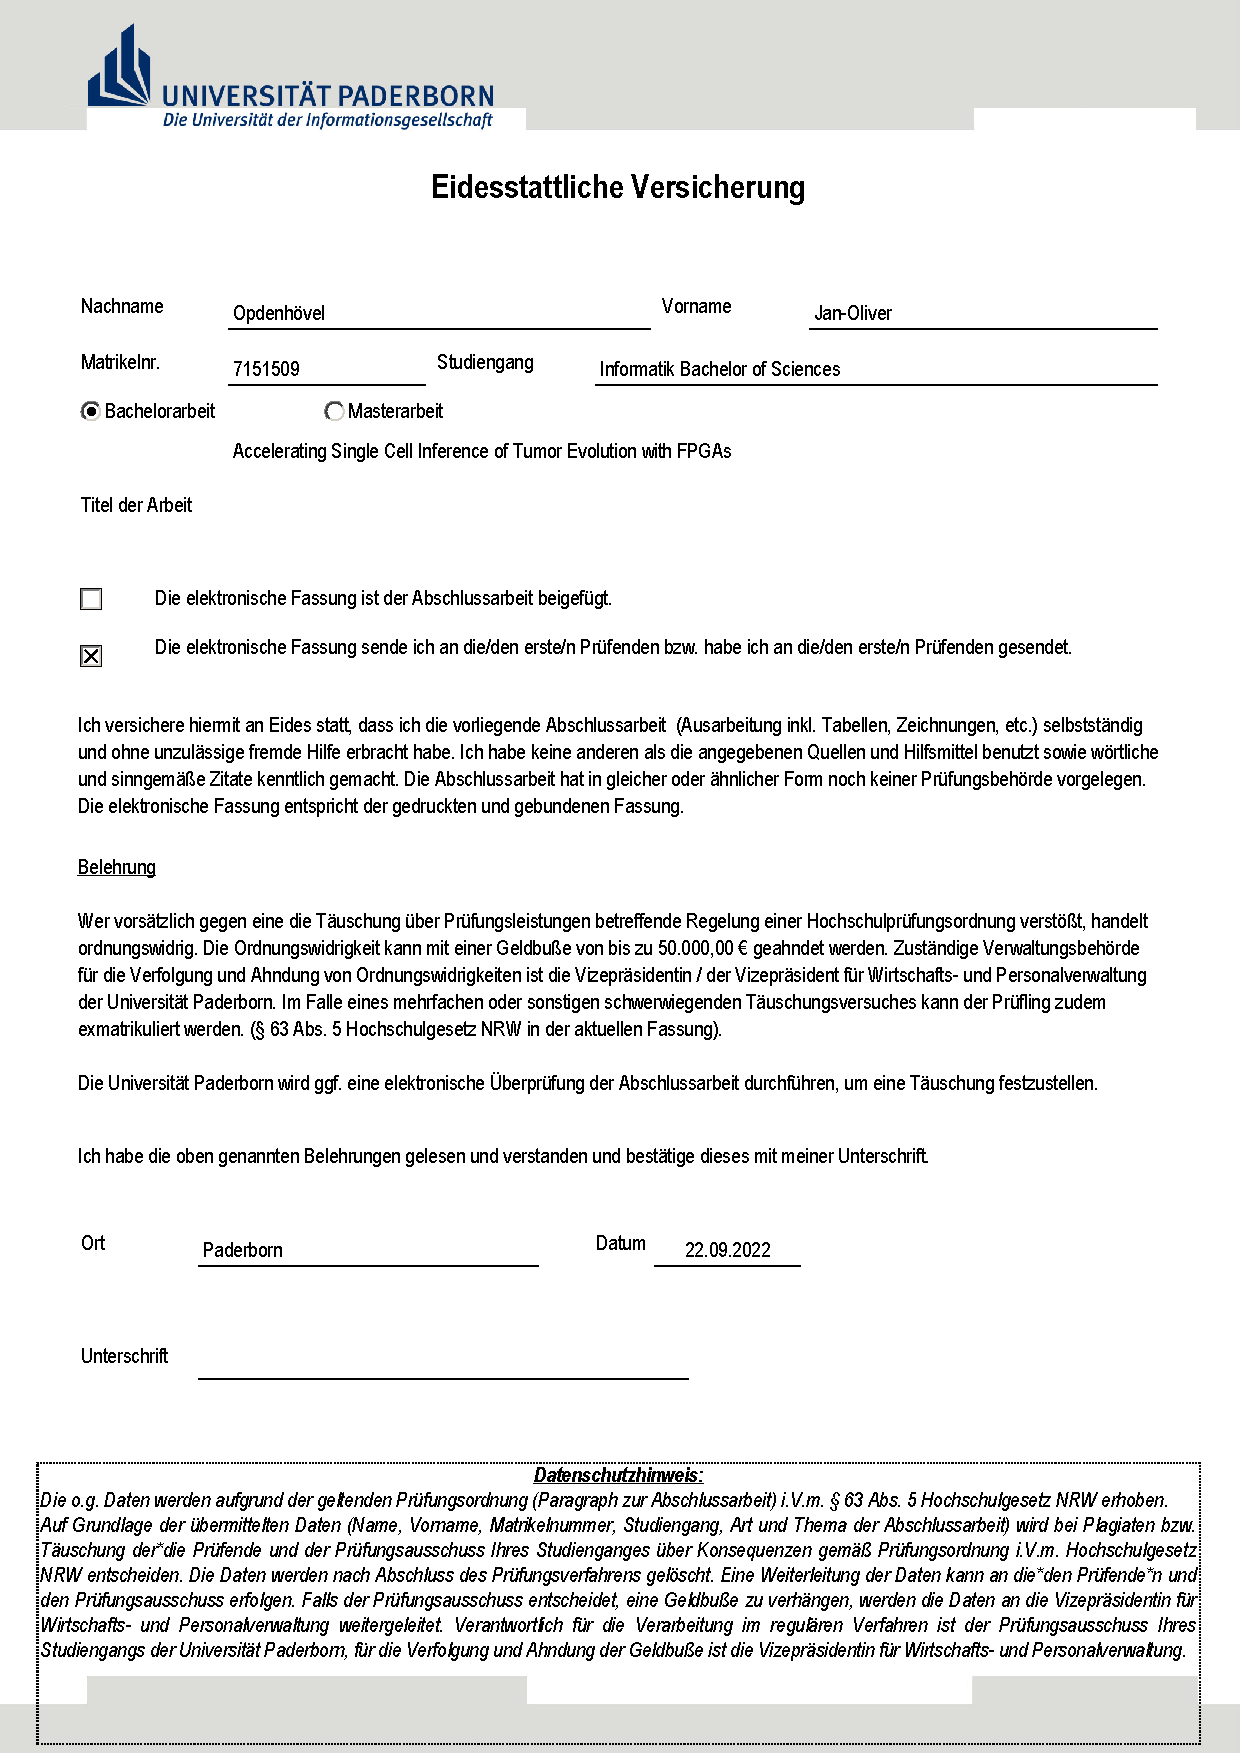
\includepdf[pages={1}]{pretext/EidesstattlicheVersicherung-fixed.pdf}
\cleardoublepage
\vspace*{\fill}
\begin{abstract}
	\acs{SCITE} is a randomized \acl{MCMC} algorithm that computes the most likely mutation history of a set of tumor cells, given noisy input data. We have accelerated \acs{SCITE} using \acp{FPGA} by a factor of 8.63 relative to the reference implementation, using the Intel Stratix 10 \acp{FPGA} at the Noctua 2 supercomputer and Intel oneAPI. We also empirically verified the solution quality using the \acl{TOST} procedure. This performance performance has been achieved mostly by pipelining the chain step operation, which required introducing \ac{FPGA}-specific algorithms to query and update data structures, restructuring the score computation function, isolating the random number generation, as well as building an optimized input/output/feedback system. The remaining bottlenecks are the score computation function due its high number of required operations and the random number generation due to a high-latency data dependency. In this thesis, we describe all our optimizations, show their correctness and how they affect the design's performance.

\end{abstract}
\acresetall
\vspace*{\fill}
\emptypage

\tableofcontents % prints the table of contents


%%%%%%%%%
% the contents of your thesis go into file body.tex
%%%%%%%%%
\chapter{Introduction}
\label{ch:introduction}

\section{Motivation and Goal of the Thesis}

Cancer is a widespread and often lethal disease\cite{10.1001/jamaoncol.2021.6987} where body cells mutate in a way that increases their cell division speed as well as their lifetime while also evading natural cancer prevention mechanisms. There are many possible treatment methods like surgery, chemotherapy, or radiation therapy, but their effectiveness often depends on the exact type of tumor. The complexity of choosing the correct therapy is increased since the tumor cells may mutate again and form metastases in different parts of the body. These developments however can be anticipated by analysing the genome of a tumor and finding new, emerging subclones that may require different treatments even before they are dominant.

Bulk sequencing of tumor cells and analysing the found mutations is already widely used, but often misses out on smaller, upcoming variants since they are averaged out in the mass of cells. Therefore, research has been done to utilise single cell sequencing. With this technique, the exact genome of individual cells can be identified and compared against other cells. However, it also comes with high error rates and parts of a cell's genome are often lost during the process. It is therefore impossible to compute an exact phylogenetic tree with this data. Instead, one has to resort to find the most plausible one.

One algorithm to compute the most likely phylogeny from a set of erroneous cell genomes is \ac{SCITE}\cite{tree2016}. The original authors provided a functional, but rather unoptimized implementation of their algorithm. While I know of an optimized but unpublished implementation of \ac{SCITE} for CPUs, there has not been an efficient implementation for \acp{FPGA} to my knowledge. \acp{FPGA} are computer chips that contain a lattice of logic, computation, and memory units that are connected via programmable connections. They basically emulate a complete computer chip and have already been used extensively for chip prototyping and verification. In recent years they have also become interesting as computation accelerators for \ac{HPC} clusters due to their low power consumption compared to their performance. However, developing efficient \ac{FPGA} designs is tedious since compiling them often takes multiple hours and naive designs are often multiple orders of magnitudes worse than optimized ones. \todo[inline]{Add notes about usage}

However, with the introduction of Intel's oneAPI, it has become possible to develop \ac{FPGA} designs using C++ templates, a form of polymorphism that is very suitable for \ac{FPGA} designs: Datatypes and functions are implemented with placeholders that can be replaced with actual types and constants during compilation. When set up correctly, one can therefore implement different solutions to the same problem, integrate the different solutions in the build system, compile the different versions in parallel and evaluate the resulting designs side by side. I have already employed this method while developing StencilStream, a Generic Stencil Simulation Library for \acp{FPGA}, and it significantly improved my productivity.

My goal for this thesis is therefore to develop an efficient implementation of SCITE for \acp{FPGA} using oneAPI and the aforementioned development pattern. This implementation should be at least as fast as the original author's implementation, but possibly as fast as the optimized CPU version mentioned previously or even faster. With this, I want to showcase the increased productivity of \ac{FPGA} development with oneAPI, that even an undergraduate student can develop efficient FPGA designs in the limited amount of time of a Bachelor's Thesis.

\section{Problem Formulation}

The input is a function $D: C \times G \rightarrow \{0, 1, ?\}$, where $C$ is the set of sampled cells and $G$ is a set of genome positions. If for a cell $c \in C$ and a genome position $g \in G$ we have $D(c, g) = 1$, the genome position $g$ has been observed as mutated in cell $c$, and if we have $D(c, g) = 0$, the genome position $g$ has been observed in it's common form. There is also a third option $D(c, g) = ?$, which means that the genome position has not been found at all and no statement could be made whether it is mutated or not. As the existance of the $?$ option may indicate, this function is noisy and may contain errors. It is assumed that errors occur independently from each other and if we let $E: C \times G \rightarrow \{0, 1\}$ be the true state of the cells, we have
\begin{align*}
    \mathbb{P}(D(c, g) = 0 \mid E(c, g) = 0) &= 1 - \alpha & \mathbb{P}(D(c, g) = 1 \mid E(c, g) = 0) &= \alpha \\
    \mathbb{P}(D(c, g) = 0 \mid E(c, g) = 1) &= \beta & \mathbb{P}(D(c, g) = 1 \mid E(c, g) = 1) &= 1 - \beta
\end{align*}
for some error rates $\alpha, \beta \in (0, 1)$. Error modeling for $D(c, g) = ?$ is not given by the authors. Missing data is always ignored in probability calculations.

The goal now is to find a mutation tree, a cell attachment and error rates with a high likelihood of being correct. A mutation tree is a rooted tree $T = (G \cup \{r\}, E, r)$ where $r$ is the root of the tree and the other nodes are genome positions. It expresses that the mutation of $g \in G$ has occured after all it's ancestors, prior to it's successors and independently from all unrelated genome positions. A cell attachment is a simple function $\sigma: C \rightarrow G$ and expresses that a cell $c \in C$ has the mutation status just after $\sigma(c)$ was mutated. Therefore, a cell $c$ has mutations at all genome positions that are ancestors of $\sigma(c)$, but at no other positions. This model is sensible since the authors of \ac{SCITE} make the ``infinite sites'' assumption, which states that a genome position mutates exactly once in the complete history of the tumor and does not mutate back.

With the mutation tree $T$ and a cell attachment $\sigma$, we can now build a function $e_{(T, \sigma)}: C \times G \rightarrow \{0, 1\}$ that expresses the made statements of the cell's true mutation status. Formally, we set
\begin{align*}
    e_{(T, \sigma)}(c, g) &:= \begin{cases}
        1 & g \in \mathrm{Anc}_T(\sigma(c)) \\
        0 & \text{else} \\
    \end{cases}
\end{align*}
where $\mathrm{Anc}_T(g)$ is the set of ancestors of a genome position $g \in G$ with respect to $T$. Therefore, the likelihood of a tree and cell attachment given the observed data $d$ and the error rates $\alpha$ and $\beta$ is
\begin{align*}
    \prod_{c \in C}\prod_{g \in G} \mathbb{P}_{(\alpha, \beta)}(D(c, g) = d(c, g) \mid E(c, g) = e_{(T, \sigma)}(c, g))
\end{align*}
Since pairs of $(c, g) \in C \times G$ with $d(c, g) = ?$ are ignored, the probabilities in the product above are always set to 1. As stated before, the goal is now to find the tuple $(T, \sigma, \alpha, \beta)$ with the highest likelihood.

\section{Algorithm introduction}

\ac{SCITE} is a \ac{MCMC} algorithm. A Monte Carlo algorithm runs a random experiment that produces possible solutions to a problem and evaluates how well the generated solutions solve the problem. This operation of generating and evaluating a solution is then repeated multiple times and the result is the best solution the algorithm has encountered. In theory, it would suffice if the experiment had a probability greater than zero to produce a good solution, but in order to improve the solution quality and to reduce the required repetitions, one would use an experiment that produces the best solutions with a higher probability than worse solutions and that can be repeated quickly. As the name implies, \ac{MCMC} algorithms simulate a Markov Chain to produce solutions. The advantage of using Markov Chains is that the next sample may depend on the previous one. The algorithm may therefore introduce small changes to the solution. This is obviously faster than generating a new solution from scratch and if the current sample is already a good solution, the change may preserve some of its quality. However, a designer of a \ac{MCMC} algorithm has to make sure that the chain actually converges on the desired distribution.

\section{Previous Work}

\section{Work Schedule}
\chapter{Findings}
\label{ch:findings}

\todo[inline]{Write that the initial implementation was uneventful and unit testing helped in the process.}

\section{Ancestor Matrix Operations}

\begin{itemize}
    \item (Informally) Motivate updating the ancestor matrix instead of rebuilding it.
    \item Formalize mutation tree, reachability, mutation matrix, tree operations.
    \item Postulate update operations, proof correctness, report results
    \item Proof uniqueness of ancestor matrix
\end{itemize}
\section{Mutation Tree Scoring}

\begin{itemize}
    \item Precomputation of scores and reduction,
    \item Partial unrolling
\end{itemize}
\chapter{Testing}
\label{ch:testing}

\todo[inline]{The chapter title isn't quite accurate. We are analysing the properties of \ac{ffSCITE}, which in the case of hardware usage isn't done by testing. Ideas for a better title?}

The goal of this thesis can be summarized as implementing the \ac{SCITE} algorithm with the same solution quality as the reference implementation, but faster. We describe how we achieved this in the previous chapter \ref{ch:design}, but we also needed to verify that we met this goal. This chapter describes how we tested the solution quality of \ac{ffSCITE} using the \ac{TOST} procedure \cite{schuirmann1987comparison} and evaluated its performance using the synthesis report, benchmarking, and profiling. 

Before we can discuss the features of the final build of \ac{ffSCITE}, we need to discuss one general issue: In section \ref{sec:encoding}, we have decided to limit the maximal number of cells and genes that are processable by the compiled design to an arbitrary number. Therefore, we need to decide on a number of cells and genes for our final design. Our final build of \ac{ffSCITE} supports 64 cells and 63 genes, which is equivalent to mutation trees with 64 nodes. This covers all but one of the example datasets that is bundled with the source code of \ac{SCITE} and compiling the design for 128 cells and 128 genes leads to internal compiler errors we were not able to resolve in time. Lastly, targeting 64 cells and 63 genes also leads to reasonable resource usage which we will discuss later in this section. Therefore, we decided to continue with this input size.

In this chapter, we will first discuss the properties that can be evaluated using the final synthesis report, namely the hardware usage and loop characteristics. (Dynamic profiling). Lastly, we evaluate the solution quality of \ac{ffSCITE}, for which we have to introduce and execute a statistical test. The most important results of these sections are listed in table \ref{tab:quickfacts} for quick look-up.

\begin{table}
    \centering
    \begin{tabular}{r|l}
        \textbf{Metric}                     & \textbf{Value} \\
        \hline
        Max. no. of cells                   & 64 \\
        Max. no. of genes                   & 63 \\
        Clock frequency                     & 295.83 MHz \\
        Macro-pipeline capacity             & 6 states \\
        Device utilization (Kernels + DSP)  & 69\% \acsp{LUT}
    \end{tabular}
    \caption{Quick facts about the final \ac{ffSCITE} build.}
    \label{tab:quickfacts}
\end{table}

\section{Hardware usage}

Tables \ref{tab:abs-usage} and \ref{tab:rel-usage} list the hardware usages of the different kernels for our target \ac{FPGA} and input sizes. The overall design is very logic-intensive, which makes sense since most of the work is done with custom logic and very few floating-point operations. Of all individual components indicated in the design schematic (Figure \ref{fig:design_schematic}), the tree score mapping loop is the heaviest and makes up roughly 37.7\% and 37.5\% of the entire design's \ac{LUT} and \ac{FF} usage, respectively. This makes sense since it is a three-dimensional loop where the inner-most loop is completely unrolled (i.e. unroll factor 64) and the middle loop is eight times partially unrolled, as we have discussed in section \ref{sec:scoring}. Therefore, the inner loop's body is replicated 512 times, which leads to the reported resource usage. The next-biggest component is the change proposer with 33.3\% and 25\% of the design's \ac{LUT} and \ac{FF} usage, respectively. This resource usage is independent of the input size since it is dominated by the \ac{URNG} executions which involve a 64-bit integer multiplication and remainder operation; Compiling the design for smaller input sizes yields similar resource usages for the change proposer.

It may be possible to further unroll the middle loop of the tree score mapping loop and double its potential throughput and hardware usage, and an extension to bigger inputs may be possible if the compiler issues were resolved. However, experience has shown us that designs with a total logic usage over 75\% start to run into issues regarding compilation times and clock frequencies. Therefore, we decided to settle with this configuration. It is however impossible to replicate the entire design another time to double the potential performance.

\begin{table}
    \centering
    \begin{tabular}{l|l|l|l|l|l}
        &                           \textbf{LUTs}&      \textbf{FFs} &      \textbf{RAMs} & \textbf{MLABs} &    \textbf{DSPs} \\
        \hline
        Pipe resources &            90 &                1.9k &              0  &            0  &                0 	\\
        IO-Kernel &                 12.3k &             3.9k &              180 &           431 &               1.5 \\
        Tree Scorer &               537.4k &            817.7k &            2.0k &          1.6k &              340.5  \\
        - Find Parent Loop &        34.1k &         	48.2k &	            22 &            46 &                0 \\
        - Tree Update Loop &        54.1k &             61.5k &             131 &           32 &                0 \\
        - Tree Score Mapping Loop & 313.4k &            439.9k &            332 &           262 &               72 \\
        - Tree Score Reduction Loop& 31.5k &            70.3k &             309 &           32 &                0 \\
        Change Proposer &           274.1k &            307.4k &            114 &           299 &               40.5 \\
        \hline
        \textbf{Kernels} &          \textbf{843.8k} &   \textbf{1.2M} &     \textbf{2.4k} &	\textbf{2.4k} &     \textbf{382.5} \\
        \textbf{Static Partition} & \textbf{455.2k} &   \textbf{910.5k} &   \textbf{2627} &	\textbf{0} &        \textbf{1.0k}	
    \end{tabular}
    \caption{Hardware usage of \ac{ffSCITE} in absolute numbers, supporting up to 64 cells and 63 genes, as reported in the ``Area Analysis'' report.}
    \label{tab:abs-usage}
\end{table}

\begin{table}
    \centering
    \begin{tabular}{l|l|l|l|l|l}
        &                               \textbf{LUTs}&  \textbf{FFs} &  \textbf{RAMs} & \textbf{MLABs} &    \textbf{DSPs} \\
        \hline
        Pipe resources &                <1\% &          <1\% &          0\% &           0\% &               0\%	\\
        IO-Kernel &                     1\% &           1\% &           2\% &           <1\% &              <1\% \\
        Tree Scorer &                   29\% &          22\% &          17\% &          2\% &               6\% \\
        - Find Parent Loop &            2\% &           1\% &           <1\% &          <1\% &              0\% \\
        - Tree Update Loop &            3\% &           2\% &           1\% &           <1\% &              0\% \\
        - Tree Score Mapping Loop &     17\% &          12\% &          3\% &           0\% &               1\% \\
        - Tree Score Reduction Loop&    2\% &           2\% &           3\% &           <1\% &              0\% \\
        Change Proposer &               15\% &          8\% &           1\% &           <1\% &              1\% \\
        \hline
        \textbf{Kernels} &              \textbf{45\%} & \textbf{32\%} & \textbf{20\%} & \textbf{3\%} &      \textbf{7\%} \\
        \textbf{Static Partition} &     \textbf{24\%}&  \textbf{24\%} & \textbf{22\%} & \textbf{0\%} &      \textbf{18\%}	
    \end{tabular}
    \caption{Hardware usage of \ac{ffSCITE} relative to the resources available on Intel Stratix 10 GX 2800 \acp{FPGA}, supporting up to 64 cells and 63 genes, as reported in the ``Area Analysis'' report.}
    \label{tab:rel-usage}
\end{table}


\section{Throughput Benchmark}

\begin{itemize}
    \item Describe benchmark setup and results
\end{itemize}
\section{Quality Testing}

We first look at the solution quality. Although we used unit tests to verify individual components, this does not suffice to verify that the entire application behaves correctly. This however can not be done by deterministic tests since \ac{SCITE} is a stochastic algorithm: Given different seeds, it produces different solutions which may or may not be perfect. We also could not implement \ac{ffSCITE} as a bit-exact copy of \ac{SCITE}, especially since we could not use the same \ac{URNG} as the reference implementation. We, therefore, needed to introduce a statistical test that verifies that given the same input, both \ac{SCITE} and \ac{ffSCITE} produce equivalent outputs. In this section, we discuss how we designed the test and what the results are.

\subsection{Methods}

Let $C$ be the set of considered cells, $G$ be the set of considered genes, and $d \in \{0,1,2\}^{|C| \times |G|}$. We model the output mutation trees of \ac{SCITE} and \ac{ffSCITE} given the inputs $C$, $G$, and $d$ as the random variables $T_\mathrm{SCITE}$ and $T_\mathrm{ffSCITE}$. We again work with log-likelihoods since the true likelihood scores for practically sized inputs are too close to 0 to express them using 64-bit floating-point numbers. Therefore, we intuitively want to find evidence for the statement $\mathbb{E} \log\Lambda_d(T_\mathrm{SCITE}) = \mathbb{E} \log\Lambda_d(T_\mathrm{ffSCITE})$. However, classical hypothesis tests only able to provide evidence for inequality statements like $\mathbb{E} \log\Lambda_d(T_\mathrm{SCITE}) < \mathbb{E} \log\Lambda_d(T_\mathrm{ffSCITE})$. This is not what we aim for and not what we claim. Therefore, we need a different approach.

In the field of clinical studies, non-inferiority and equivalence trials are a common tool. There, these kinds of trials ``are intended to show that the effect of a new treatment is not worse than that of an active control by more than a specified margin.'' \cite{snapinn2000noninferiority} Although there are some complications with using non-inferiority trails for drug testing as pointed out by Snapinn \cite{snapinn2000noninferiority}, these complications do not apply to our scenario. The exact procedure that we use is called \acf{TOST}, which was introduced by Donald J Schuirmann in 1987 \cite{schuirmann1987comparison} and it requires its designer to set an equivalence margin $\delta$, where absolute differences below this margin are considered negligible. Then, our alternative and null hypotheses are:
\begin{align*}
    H_1&: \mathbb{E} |\log\Lambda_d(T_\mathrm{SCITE}) - \log\Lambda_d(T_\mathrm{ffSCITE})| < \delta \\
    H_0&: \mathbb{E} |\log\Lambda_d(T_\mathrm{SCITE}) - \log\Lambda_d(T_\mathrm{ffSCITE})| \geq \delta \\
    &\Leftrightarrow \mathbb{E} \left(\log\Lambda_d(T_\mathrm{SCITE}) - \log\Lambda_d(T_\mathrm{ffSCITE})\right) \leq - \delta \vee \mathbb{E} \left(\log\Lambda_d(T_\mathrm{SCITE}) - \log\Lambda_d(T_\mathrm{ffSCITE})\right) \geq \delta
\end{align*}
Once our hypotheses are established, we can execute a one-sided t-test for each half of $H_0$ and if both fail, we have provided evidence for the equivalence for \ac{ffSCITE} and \ac{SCITE}.

Intuitively, we want to pick $\delta$ as close to 0 as possible, but we still want to provide a reasonable margin. One of the most natural choices for $\delta$ might be the maximum likelihood difference from one chain step to the next. If ffSCITE were equivalent to SCITE within this margin, it would mean that ffSCITE may just have missed the last chain step to the optimal solution out of bad luck, which one could deem as negligible. However, the effects of a chain step may be chaotic since the cell-node attachments are recomputed and might change after every operation. These attachment changes not only depend on the mutation tree, but also on the error probabilities and the observed mutation data. As of this writing, we do not have enough understanding of a chain step's effect on the state likelihood, and we also did not have the time to develop it. Therefore, we need to take a step back and remember that we have assigned the likelihood score in definition \ref{def:likelihood} to mutation matrices, not to mutation trees. These are only a tool to ease the proposal of mutation matrices. If we, therefore, consider a maximum-likelihood mutation matrix $e \in \{0,1\}^{|C| \times |G|}$, then the smallest logical deviation from it is a single bit-flip. Therefore, we have decided to set our $\delta$ to the maximum log-likelihood difference induced by a bit-flip, which is 
\begin{align*}
    \delta :=\max\{|\log(\alpha) - \log(1-\beta)|, |\log(\beta) - \log(1-\alpha)|\}
\end{align*}
according to lemma \ref{lem:bitflip}, where $\alpha$ and $\beta$ are the probabilities for false positives and negatives, respectively.

\begin{lemma}
    \label{lem:bitflip}
    Let $C$ be the set of considered cells, $G$ be the set of considered genes, $d \in \{0,1,2\}^{|C| \times |G|}$, and $e, e' \in \{0,1\}^{|C| \times |G|}$ where $e$ is arbitrary and $e'$ is defined as:
    \begin{align*}
        e'_{c,g} &:= \begin{cases}
            \overline{e_{c,g}} & c = x \wedge g = y \\
            e_{c,g} & \text{else}
        \end{cases}
    \end{align*}
    for some $x \in C$, $y \in G$. In other words, $e'$ is a version of $e$ where the bit at position $(x,y)$ is flipped. Let also $\alpha, \beta \in [0,1]$ be the probabilities of false positives and negatives, respectively. Then, we have:
    \begin{align*}
        |\log\Lambda_d(e) - \log\Lambda_d(e')| &\leq \max\{|\log(\alpha) - \log(1-\beta)|, |\log(\beta) - \log(1-\alpha)|\}
    \end{align*}
    where $\Lambda_d$ is the likelihood function of definition \ref{def:likelihood}. In other words, the difference in log-likelihood induced by a single bit flip is equal to or less than $\max\{|\log(\alpha) - \log(1-\beta)|, |\log(\beta) - \log(1-\alpha)|\}$.
\end{lemma}

\begin{proof}
    First of all, we should remark that we have
    \begin{align*}
        \log\Lambda_d(e) &= \sum_{c \in C} \sum_{g \in G} \log\lambda(d_{c,g}, e_{c,g}) \\
        \Rightarrow |\log\Lambda_d(e) - \log\Lambda_d(e')| &= |\log\lambda(d_{x,y}, e_{x,y}) - \log\lambda(d_{x,y}, e'_{x,y})| \\
        &= |\log\lambda(d_{x,y}, e_{x,y}) - \log\lambda(d_{x,y}, \overline{e_{x,y}})|
    \end{align*}
    If we have $d_{x,y} = 2$, we therefore have
    \begin{align*}
        |\log\Lambda_d(e) - \log\Lambda_d(e')| &= |\log(1) - \log(1)| = 0
    \end{align*}
    Our lemma is therefore true in this case and we can assume $d_{x,y} \neq 2 \Rightarrow d_{x,y} \in \{0,1\}$. We now have four cases:
    \begin{itemize}
        \item $d_{x,y} = 0, e_{x,y} = 0$: We then have
        \begin{align*}
            |\log\Lambda_d(e) - \log\Lambda_d(e')| = |\log\lambda(0,0) - \log\lambda(0,1)| = |\log(1-\alpha) - \log(\beta)|
        \end{align*}
        \item $d_{x,y} = 0, e_{x,y} = 1$: We then have
        \begin{align*}
            |\log\Lambda_d(e) - \log\Lambda_d(e')| = |\log\lambda(0,1) - \log\lambda(0,0)| = |\log(\beta) - \log(1-\alpha)|
        \end{align*}
        \item $d_{x,y} = 1, e_{x,y} = 0$: We then have
        \begin{align*}
            |\log\Lambda_d(e) - \log\Lambda_d(e')| = |\log\lambda(1,0) - \log\lambda(1,1)| = |\log(1-\beta) - \log(\alpha)|
        \end{align*}
        \item $d_{x,y} = 1, e_{x,y} = 1$: We then have
        \begin{align*}
            |\log\Lambda_d(e) - \log\Lambda_d(e')| = |\log\lambda(1,1) - \log\lambda(1,0)| = |\log(\alpha) - \log(1-\beta)|
        \end{align*}
    \end{itemize}
    $|\log\Lambda_d(e) - \log\Lambda_d(e')|$ is always equal to or less than the maximum of all these cases and we therefore have
    \begin{align*}
        |\log\Lambda_d(e) - \log\Lambda_d(e')| &\leq \max\{|\log(\alpha) - \log(1-\beta)|, |\log(\beta) - \log(1-\alpha)|\}
    \end{align*}
\end{proof}

Let us summarize our quality testing method: First, we have randomly generated 64 observed mutation data matrices considering 64 cells and 63 genes, with a probability of $\alpha := 10^{-6}$ for false positives, $\beta := 0.25$ for false negatives, and $0.25$ for missing data. Then, we ran 6 chains á 1,000,000 steps on these mutation data matrices, using both \ac{SCITE} and \ac{ffSCITE}, and stored the resulting max-likelihood mutation trees. This input size of 64 cells and 63 genes is the maximum our build of \ac{ffSCITE} can support, and we chose the number of input sets, chains, and steps as a compromise between expressiveness and execution time since we wanted to run the same experiment multiple times during development to continuously check our design. The error probabilities are however arbitrary since we did not have realistic numbers available or the time to research them. After the execution was completed, we used a Python script to compute the differences in log-likelihood produced by \ac{SCITE} and \ac{ffSCITE} for the same inputs and used SciPy to run one-sided t-tests against the parts of our null-hypothesis with a significance level of 0.01. Therefore, the significance level of the entire test is 0.02.

\subsection{Results}

Out of the 64 inputs, \ac{SCITE} and \ac{ffSCITE} achieved the same likelihoods for 47 inputs. \ac{ffSCITE} scored better in 10 cases, and \ac{SCITE} scored better in 7 cases. Interestingly, all encountered differences are multiples of our $\delta$, which is defined as the maximum difference induced by a bit-flip. Therefore, we plotted the number of outputs with a certain log-likelihood difference in multiples of $\delta$ or bit-flips in figure \ref{fig:likelihood_differences}. Another notable finding is that \ac{SCITE} and \ac{ffSCITE} never deviate by more than two bit-flips and the mean difference between \ac{SCITE}'s and \ac{ffSCITE}'s log-likelihood score is $0.65$. Lastly, the p-value for the test of $\mathbb{E} \left(\log\Lambda_d(T_\mathrm{SCITE}) - \log\Lambda_d(T_\mathrm{ffSCITE})\right) \leq - \delta$ is $p_- \approx 9.47 \cdot 10^{-21}$ and the p-value for the test of $\mathbb{E} \left(\log\Lambda_d(T_\mathrm{SCITE}) - \log\Lambda_d(T_\mathrm{ffSCITE})\right) \geq \delta$ is $p_+ \approx 7.87 \cdot 10^{-19}$. Therefore, we have to reject $H_0$ and have provided evidence that \ac{ffSCITE} and \ac{SCITE} produce solutions of equivalent quality.

\begin{figure}
    \centering
    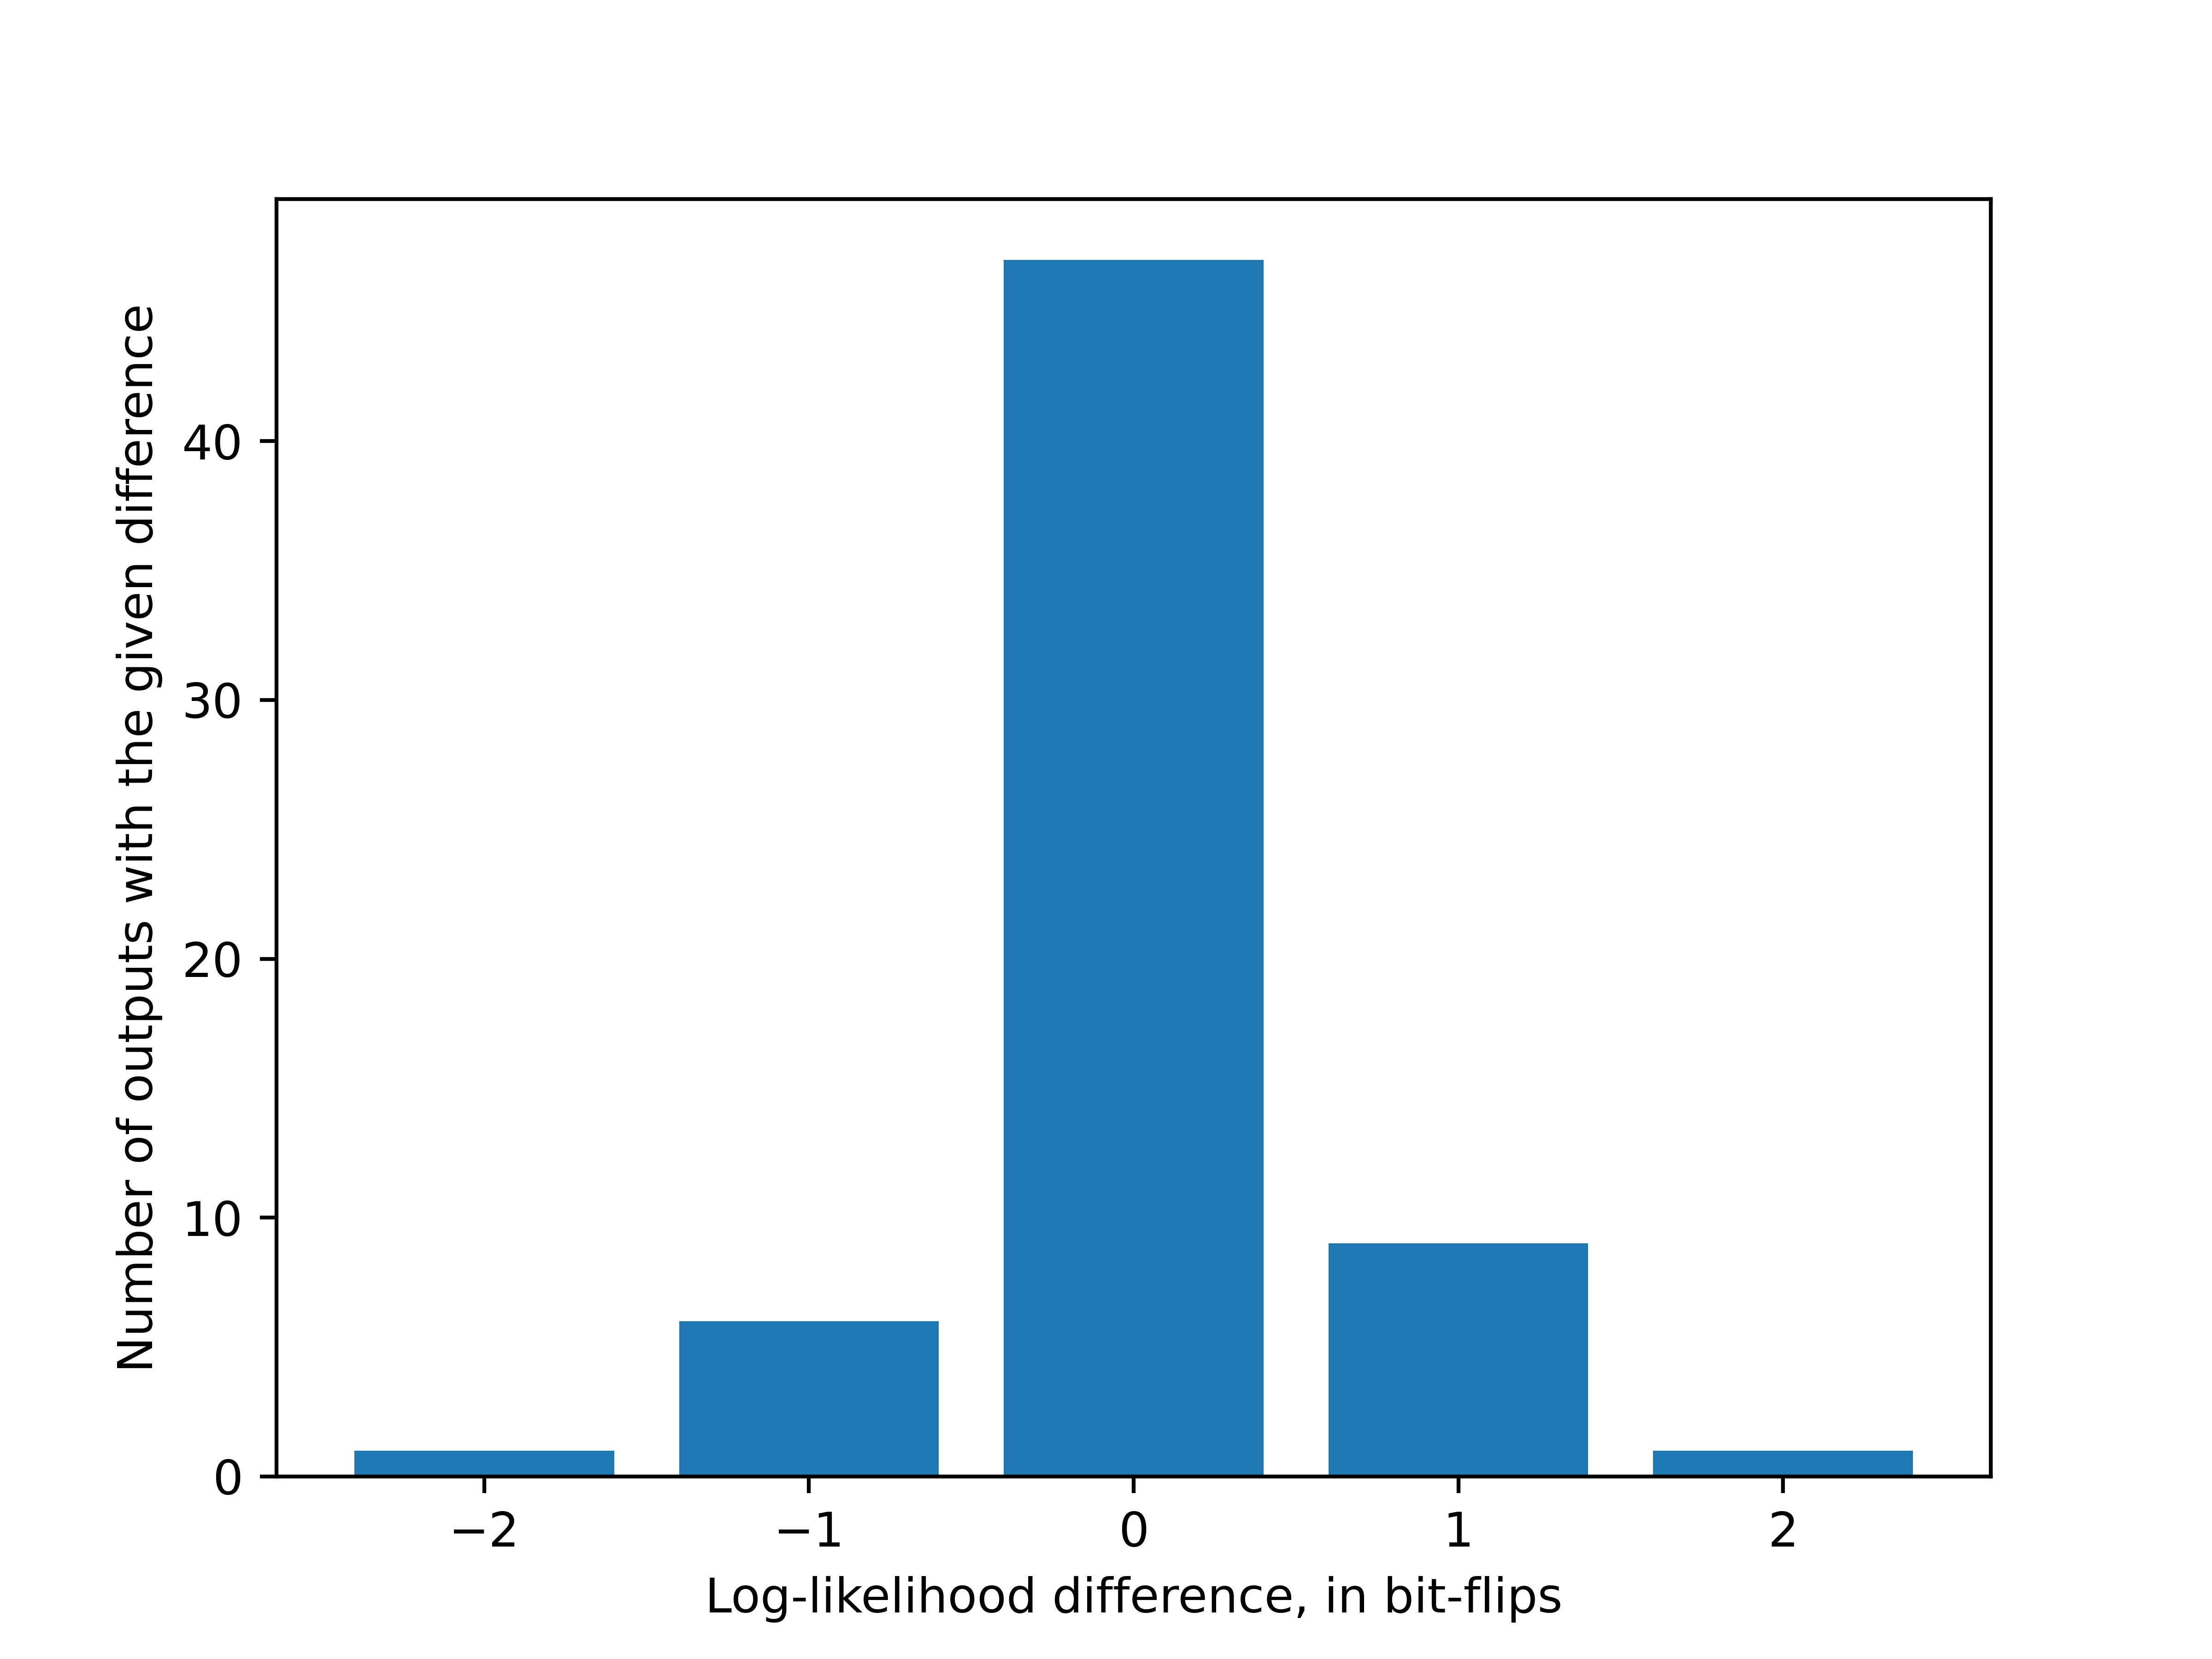
\includegraphics[width=0.75\textwidth]{figures/likelihood_differences.png}
    \caption{Accumulated differences in log-likelihood between solutions provided by \ac{SCITE} and \ac{ffSCITE}. A positive difference means that \ac{ffSCITE} has provided a better solution than \ac{SCITE}, and a negative difference means the opposite.}
    \label{fig:likelihood_differences}
\end{figure}
\chapter{Conclusion}
\label{ch:conclusion}

\ac{ffSCITE} reaches the goal of being an implementation of the \ac{SCITE} algorithm for \acp{FPGA} with higher throughput than the reference implementation by Jahn et al. \cite{tree2016}. This algorithm computes the most likely mutation history of a group of tumor cells, given noisy information about their mutation status.

Our biggest contribution is an improvement to the mutation tree encoding: The reference implementation uses parent vectors as the canonical data structure, which contain the parent of every node in the tree. However, it also uses ancestor matrices to analyze the mutation tree, which denote whether there is a path from one node in the tree to another. These ancestor matrices are constructed from parent vectors and this operation is not practical on \acp{FPGA}. We, therefore, developed algorithms to reconstruct the mutation tree from an ancestor matrix and to compute the resulting ancestor matrix of a tree modification based on the old one. These algorithms are impractical on \acp{CPU} but work well on \acp{FPGA} due to their flexibility regarding custom logic, and due to this contribution, our implementation can work exclusively on ancestor matrices and avoid constructing ancestor matrices on the device.

Additionally, we reformulated the algorithm to compute a mutation tree's likelihood: The reference implementation uses two different implementations with different precisions to improve performance, but since \ac{ffSCITE} would not benefit from computing it twice, we based our formulation on the fast method. The likelihood computation algorithm can be described as a mapping step followed by a two-dimensional reduction. The original formulation executed the reductions together with the mapping operation, which created too many loop-carried dependencies and resulted in a structurally underperforming design. We, therefore, split the mapping and the two reductions into separate loops and used loop unrolling to improve the loop's throughput at the cost of higher resource usage.

Lastly, we also dealt with issues regarding random number generation: We used \acfp{URNG} and distribution algorithms from the C++ standard library and Intel's oneDPL to reduce development time. While these implementations work correctly on \acp{FPGA}, they were originally designed for \acp{CPU}. We especially faced issues with our \ac{URNG}, the Minstd \ac{URNG} \cite{park1988random}, since it uses 64-bit integer multiply and remainder operations. These operations have a high resource usage and latency, and since their output is supposed to appear random, they create a data dependency that leads to an increased \acf{II} for the loop that uses them. Therefore, we isolated the random draws into a separate kernel and reduced the \ac{II} of its main loop to a level below the current bottleneck.

The previous optimizations resulted in a macro-pipeline where different components work independently from one another to execute a chain step. This pipeline needs to be filled at all times to maximize the mean throughput. We did this by filling the pipeline with initial chain states once, feeding the emitted states back after a chain step, and replacing them with new initial states once the chains are complete. Our scheme ensures that the pipeline is always filled and also simplifies and minimizes interactions with off-chip memory, which additionally reduces compilation times and potentially increases energy efficiency.

The resulting chip design utilizes up to 69\% of the resources available on our target device, a Bittware 520N card with an Intel Stratix 10 GX 2800 \ac{FPGA}. Our design achieves a constant throughput of 577.8 thousand chain steps per second and is bottlenecked by the mapping step of the likelihood computation, as we have predicted based on the synthesis report. Compared to the reference implementation run on one of Noctua 2's compute nodes, our implementation has up to 8.6 times higher throughput. However, our implementation likely has a lower throughput than the one by Ernst et al. \cite{ernst2020Performance}, which is an optimized version of the \ac{CPU} reference implementation.

Our last goal was to verify that our implementation produces results of similar quality compared to the reference implementation. Since the \ac{SCITE} algorithm is not deterministic and our optimizations did not allow us to implement a bit-perfect copy of the reference, we had to use a statistical test to verify our solution quality. We used the \acf{TOST} procedure \cite{schuirmann1987comparison} to define an equivalence test that compares two implementations of the \ac{SCITE} algorithm, and our implementation is equivalent to the reference implementation with a significance level of 2\%.

\section{Open directions}
\label{sec:open_directions}

\todo[inline]{Note that time was lacking}

\begin{itemize}
    \item Feature: Homocygous/Heterocygous mutations
    \item Feature: Sum score
    \item Feature: Finding the most-likely beta
    \item Feature: Co-optimal trees
    \item Feature: Sampling from posterior distribution
    \item New Feature: Continuous likelihood outputs
    \item New Feature/Optimization: Multi-Input
    \item Optimization: Customized RNG and distributions (Lower resource usage, increase throughput)
    \item Optimization: Replicate MCMC step (increase throughput, requires pipelined chain step loop)
    \item Optimization: Transpose ancestor matrix (simplify memory access pattern, increase scalability)
    \item Exploration: Energy efficiency
\end{itemize}

% include the bibliography, and add it as a chapter the table of contents
\newpage
\addcontentsline{toc}{chapter}{Bibliography}
\bibliographystyle{alpha}
\bibliography{literature.bib}


%%%%%%%%%
% the appendices of your thesis go into file appendix.tex
%%%%%%%%%
\appendix



\end{document}
